\section{Einleitung}\label{sec:einleitung}
Innovationen entstehen aus Ideen. Ideen gibt es sehr viele. Doch nicht jede Idee ist für die 
Umsetzung geeignet. Ein Beispiel ist ein Produkt eines bekannten Zahnpastaherstellers. 
Die \textit{Beef Lasagne} von Colgate konnte sich nicht am Markt durchsetzen. 
Vermutlich zielte Colgate mit der Vermarktung der Lasagne ein neues Marktgebiet an. 
Leider wurden die Kriterien für die Bewertung nicht gut gewählt, denn das Produkt passte nicht Unternehmens-Image.
Dies hatte zur Folge, dass sich das Produkt nicht verkaufte und sich als Marketing-Flop herausstellte.
\begin{figure}[ht]
	\centering
	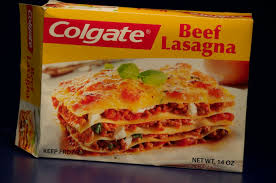
\includegraphics[width=6cm]{colgate.jpg}
	\caption{Beef Lasagne von Colgate}
	\label{img:colgate}
\end{figure}
Dieses Beispiel zeigt, wie wichtig es ist, Ideen anhand verschiedener Kriterien zu bewerten. 
In dieser Seminararbeit werden die Definitionen von Schawel-Billing und Zephram erläutert. Diese lassen sich sehr gut kombinieren. 
Anhand von zwei Praxisbeispielen aus der Abteilung \ac{sac} werden Anwendungsfälle dargestellt und die  
Kriterien zur Ideenbewertung beschrieben. 
